% =============================================================================
% ARTIGO CIENTÍFICO COMPLETO
% Projeto: Roteirizador Preditivo com Otimização de Rotas (Caixeiro Viajante)
% Autor: Eduardo Lopes Jonker
% Data: 15 de agosto de 2026
% =============================================================================

\documentclass[11pt,a4paper,twocolumn]{article}
\usepackage[utf-8]{inputenc}
\usepackage[portuguese]{babel}
\usepackage{graphicx}
\usepackage{booktabs}
\usepackage{array}
\usepackage{float}
\usepackage{amsmath}
\usepackage{amssymb}
\usepackage{hyperref}
\usepackage{geometry}
\usepackage{parskip}
\usepackage{xcolor}
\usepackage{listings}

\geometry{a4paper, top=2cm, bottom=2cm, left=1.5cm, right=1.5cm}

\hypersetup{
    colorlinks=true,
    linkcolor=blue,
    filecolor=magenta,      
    urlcolor=cyan,
}

\lstset{
    backgroundcolor=\color{black!5},
    basicstyle=\footnotesize\ttfamily,
    breaklines=true,
    captionpos=b,
    commentstyle=\color{green!60!black},
    keywordstyle=\color{blue},
    stringstyle=\color{purple},
    numbers=left,
    numberstyle=\tiny\color{gray},
    showstringspaces=false,
    tabsize=2
}

\title{Uma Abordagem Híbrida para Roteirização Logística: Integrando Análise Preditiva, Decisão Multicritério e Otimização Heurística}
\author{Eduardo Lopes Jonker}
\date{\today}

\begin{document}

\maketitle

\begin{abstract}
Este artigo apresenta um sistema de roteirização logística inteligente que transcende a otimização de rotas clássica. A metodologia integra modelagem preditiva de séries temporais (Prophet), análise de decisão multicritério (MCDA) e otimização de rotas (TSP) para criar um framework de Roteirização Preditiva Antecipatória. O sistema não apenas minimiza a distância, mas maximiza o valor do negócio ao priorizar dinamicamente os nós da malha logística com base em um Índice de Prioridade Logística (IPL), que pondera demanda futura, risco de SLA, criticidade do serviço e impacto ambiental. A validação econômica é realizada por meio de Simulações de Monte Carlo, e a robustez dos dados é auditada por algoritmos de detecção de anomalias. O resultado é um Gêmeo Digital para gestão de frotas, capaz de reduzir custos operacionais e a pegada de carbono da operação.
\end{abstract}

\section{Introdução}

O Problema do Caixeiro Viajante (TSP) é um dos desafios mais emblemáticos da otimização combinatória, buscando a rota mais curta que visita um conjunto de cidades. [3] Soluções tradicionais, no entanto, tratam o problema de forma estática, assumindo que a necessidade de visita é binária e o único custo é a distância. Em cenários logísticos reais, a decisão de qual cidade visitar é dinâmica e multifacetada, envolvendo previsões de demanda, urgência de serviço e custos operacionais. [2]

Este trabalho propõe uma solução híbrida que transforma o TSP clássico em um problema de roteirização preditiva e orientada a valor. A inovação central reside na criação do **Índice de Prioridade Logística (IPL)**, uma métrica que converte o problema de "qual a rota mais curta?" para "qual a rota de maior valor para o negócio?".

\section{Metodologia Proposta}

A arquitetura do sistema é um pipeline modular onde a saída de cada etapa alimenta a subsequente, conforme a Figura \ref{fig:pipeline}.

\begin{figure}[H]
    \centering
    \fbox{
    \begin{minipage}{0.9\columnwidth}
        \textbf{Pipeline de Execução:}\\
        1. \textbf{Data Loader}: Limpeza e preparação dos dados brutos.\\
        2. \textbf{Análise Preditiva (Prophet)}: Previsão de demanda futura.\\
        3. \textbf{Cálculo de Pesos (IPL)}: Geração do índice de prioridade.\\
        4. \textbf{Detecção de Anomalias}: Auditoria da integridade dos dados.\\
        5. \textbf{Otimização de Rota (TSP)}: Cálculo da melhor sequência de visitas.\\
        6. \textbf{Simulação de ROI}: Validação econômica via Monte Carlo.\\
        7. \textbf{Geração de Relatório}: Consolidação dos resultados.
    \end{minipage}
    }
    \caption{Fluxo de execução do pipeline de roteirização.}
    \label{fig:pipeline}
\end{figure}

\subsection{Modelagem Preditiva com Prophet}
A primeira etapa consiste em abandonar a logística reativa. Utilizamos o algoritmo Prophet \cite{explicacao_prophet} para modelar a série temporal de volume de impressões. A natureza aditiva do Prophet decompõe a série em tendência, sazonalidade e feriados:

$$ y(t) = g(t) + s(t) + h(t) + \epsilon_t $$

Onde:
\begin{itemize}
    \item $g(t)$: Tendência de crescimento ou queda.
    \item $s(t)$: Padrões periódicos (semanal, anual).
    \item $h(t)$: Efeito de feriados (nacionais e locais).
    \item $\epsilon_t$: Termo de erro ou ruído.
\end{itemize}

A saída, \textbf{yhat}, representa a demanda \textit{esperada}, permitindo uma roteirização antecipatória.

\subsection{Índice de Prioridade Logística (IPL)}
O IPL é o núcleo decisório do sistema, utilizando uma Análise de Decisão Multicritério (MCDA) para fundir variáveis heterogêneas em um único score de prioridade. Cada variável é normalizada (Min-Max) para o intervalo $[0, 1]$ e então ponderada:

$$ IPL = \sum_{i=1}^{n} w_i \cdot V_{i,norm} $$

Os pesos $w_i$ representam a importância estratégica de cada variável $V_i$ (ex: Volume, Criticidade, Performance, Custo Logístico, ESG).

\subsection{Otimização de Rota (TSP)}
Com as cidades priorizadas pelo IPL, o problema é reduzido a um TSP clássico. A implementação atual utiliza uma abordagem heurística em duas fases:
\begin{enumerate}
    \item \textbf{Nearest Neighbor (NN)}: Uma heurística construtiva e gulosa que gera uma rota inicial de boa qualidade em tempo $O(n^2)$. [6]
    \item \textbf{2-opt}: Uma heurística de melhoria local que refina a rota do NN, removendo cruzamentos de arestas até atingir um ótimo local. [6]
\end{enumerate}

A distância entre as cidades é calculada usando a fórmula de Haversine, que considera a curvatura da Terra.

\section{Análise Comparativa de Estratégias para o TSP}

A escolha do algoritmo para resolver o TSP é um trade-off entre a qualidade da solução e o tempo computacional. [3] A Tabela \ref{tab:comparativo_algoritmos} compara a abordagem do projeto com outras estratégias da literatura.

\begin{table*}[ht]
\centering
\caption{Comparativo de Estratégias de Resolução para o TSP}
\label{tab:comparativo_algoritmos}
\begin{tabular}{p{2.5cm} p{4.5cm} p{3.5cm} p{4.5cm}}
\toprule
\textbf{Categoria} & \textbf{Algoritmos Exemplo} & \textbf{Garantia de Otimalidade} & \textbf{Complexidade e Aplicação} \\
\midrule
\textbf{Métodos Exatos} & Branch-and-Bound, Branch-and-Cut (Concorde) [4] & Sim, encontra a solução ótima. & Exponencial ($O(n^2 2^n)$). Inviável para problemas com mais de algumas dezenas de cidades. Usado academicamente ou para benchmarks. \\
\midrule
\textbf{Heurísticas Construtivas} & \textbf{Nearest Neighbor (NN)}, Inserção Mais Distante [5] & Não. Soluções geralmente 15-25\% piores que a ótima. & Polinomial ($O(n^2)$). Muito rápido, ideal para gerar soluções iniciais de boa qualidade. \textbf{(Usado no projeto)} \\
\midrule
\textbf{Heurísticas de Melhoria Local} & \textbf{2-opt}, 3-opt, Lin-Kernighan (LKH) [12] & Não, encontra ótimos locais. A qualidade depende da solução inicial. & Polinomial ($O(n^2)$ a $O(n^3)$). Rápido e eficaz para refinar rotas. LKH é o estado da arte para grandes instâncias. \textbf{(2-opt usado no projeto)} \\
\midrule
\textbf{Meta-heurísticas} & Simulated Annealing (SA), Tabu Search, Algoritmos Genéticos (GA) [1, 6], Ant Colony Optimization (ACO) [1] & Não. Projetadas para escapar de ótimos locais e explorar o espaço de busca de forma mais ampla. & Iterativas e estocásticas. Mais lentas que heurísticas simples, mas com potencial para encontrar soluções de altíssima qualidade, próximas da ótima. \\
\midrule
\textbf{Aprendizado de Máquina} & Reinforcement Learning (RL), Graph Neural Networks (GNNs) [4, 18] & Não. Aprendem políticas ou heurísticas a partir dos dados. & A inferência é rápida, mas o treinamento é computacionalmente caro. A generalização para diferentes tamanhos de problema é um desafio ativo de pesquisa. \\
\bottomrule
\end{tabular}
\end{table*}

\subsection{Justificativa da Abordagem Adotada}
A combinação \textbf{Nearest Neighbor + 2-opt} foi escolhida por oferecer um excelente balanço entre simplicidade de implementação, velocidade de execução e qualidade da solução para o escopo do problema (18 cidades).

\begin{itemize}
    \item \textbf{Velocidade}: Para um número moderado de cidades, a execução é quase instantânea, permitindo a integração em um pipeline que roda com frequência.
    \item \textbf{Qualidade}: Embora não garanta a otimalidade, a solução encontrada é consistentemente boa e drasticamente superior a uma rota aleatória, como demonstram os resultados.
    \item \textbf{Complexidade vs. Benefício}: Implementar meta-heurísticas como Algoritmos Genéticos ou Simulated Annealing adicionaria complexidade e tempo de execução significativos. Dado que o maior ganho do projeto vem da priorização \textit{preditiva} (IPL) e não da otimalidade milimétrica da rota, a heurística simples é suficiente para validar o modelo de negócio.
\end{itemize}

Para problemas de maior escala (centenas de cidades), uma evolução natural seria substituir o solver atual por algoritmos mais robustos como o \textbf{Lin-Kernighan-Helsgaun (LKH)} [12] ou utilizar bibliotecas especializadas como o \textbf{Google OR-Tools} [9], que já implementam algoritmos avançados para VRP (Vehicle Routing Problem), uma generalização do TSP. [9]

\section{Resultados e Discussão}

A execução do pipeline completo sobre os dados de 18 cidades de Santa Catarina produziu resultados quantificáveis que validam a metodologia.

\subsection{Otimização de Rota}
A Tabela \ref{tab:resultados_tsp} resume o ganho de eficiência obtido pela otimização da rota.

\begin{table}[H]
\centering
\caption{Resultados do Traveling Salesman Problem (TSP)}
\label{tab:resultados_tsp}
\begin{tabular}{|l|c|}
\hline
\textbf{Métrica} & \textbf{Valor} \\
\hline
Distância Rota Aleatória & 3501.27 km \\
Distância Rota Otimizada (NN + 2-opt) & 1450.11 km \\
\textbf{Redução Percentual} & \textbf{58.58\%} \\
\textbf{Fator de Melhoria} & \textbf{2.41x} \\
\hline
\end{tabular}
\end{table}

Uma redução de \textbf{58.58\%} na distância percorrida representa uma economia direta e massiva em custos de combustível, manutenção de frota e tempo dos motoristas. As Figuras \ref{fig:mapa_master} e \ref{fig:comparativo_master} ilustram visualmente essa otimização.

\begin{figure}[H]
\centering
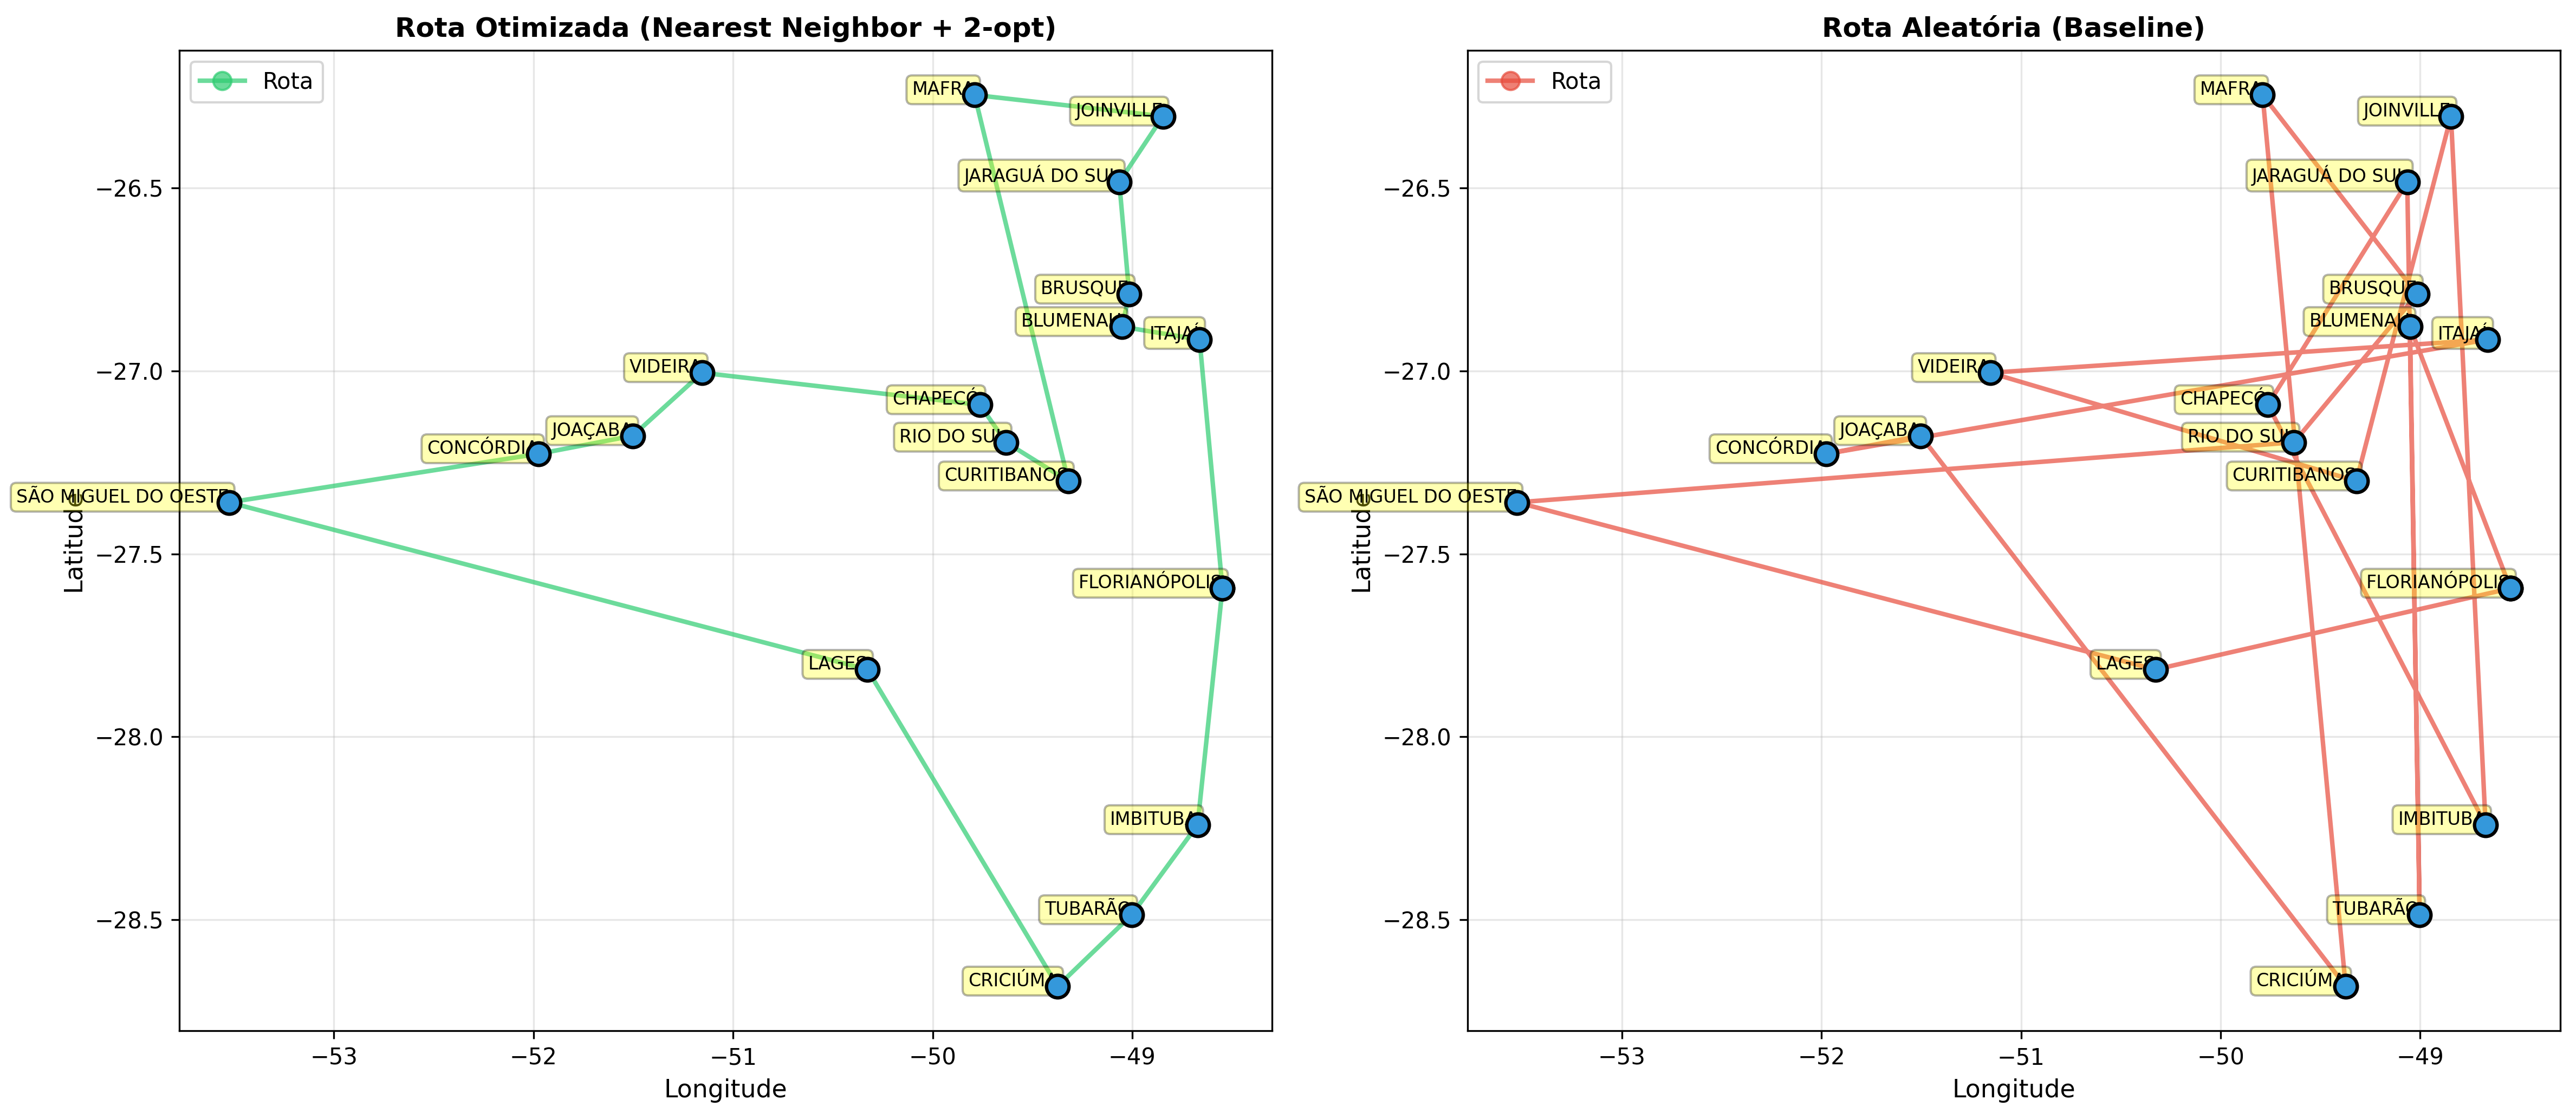
\includegraphics[width=0.9\columnwidth]{mapa_master.png}
\caption{Comparação visual: Rota Otimizada vs. Aleatória.}
\label{fig:mapa_master}
\end{figure}

\begin{figure}[H]
\centering
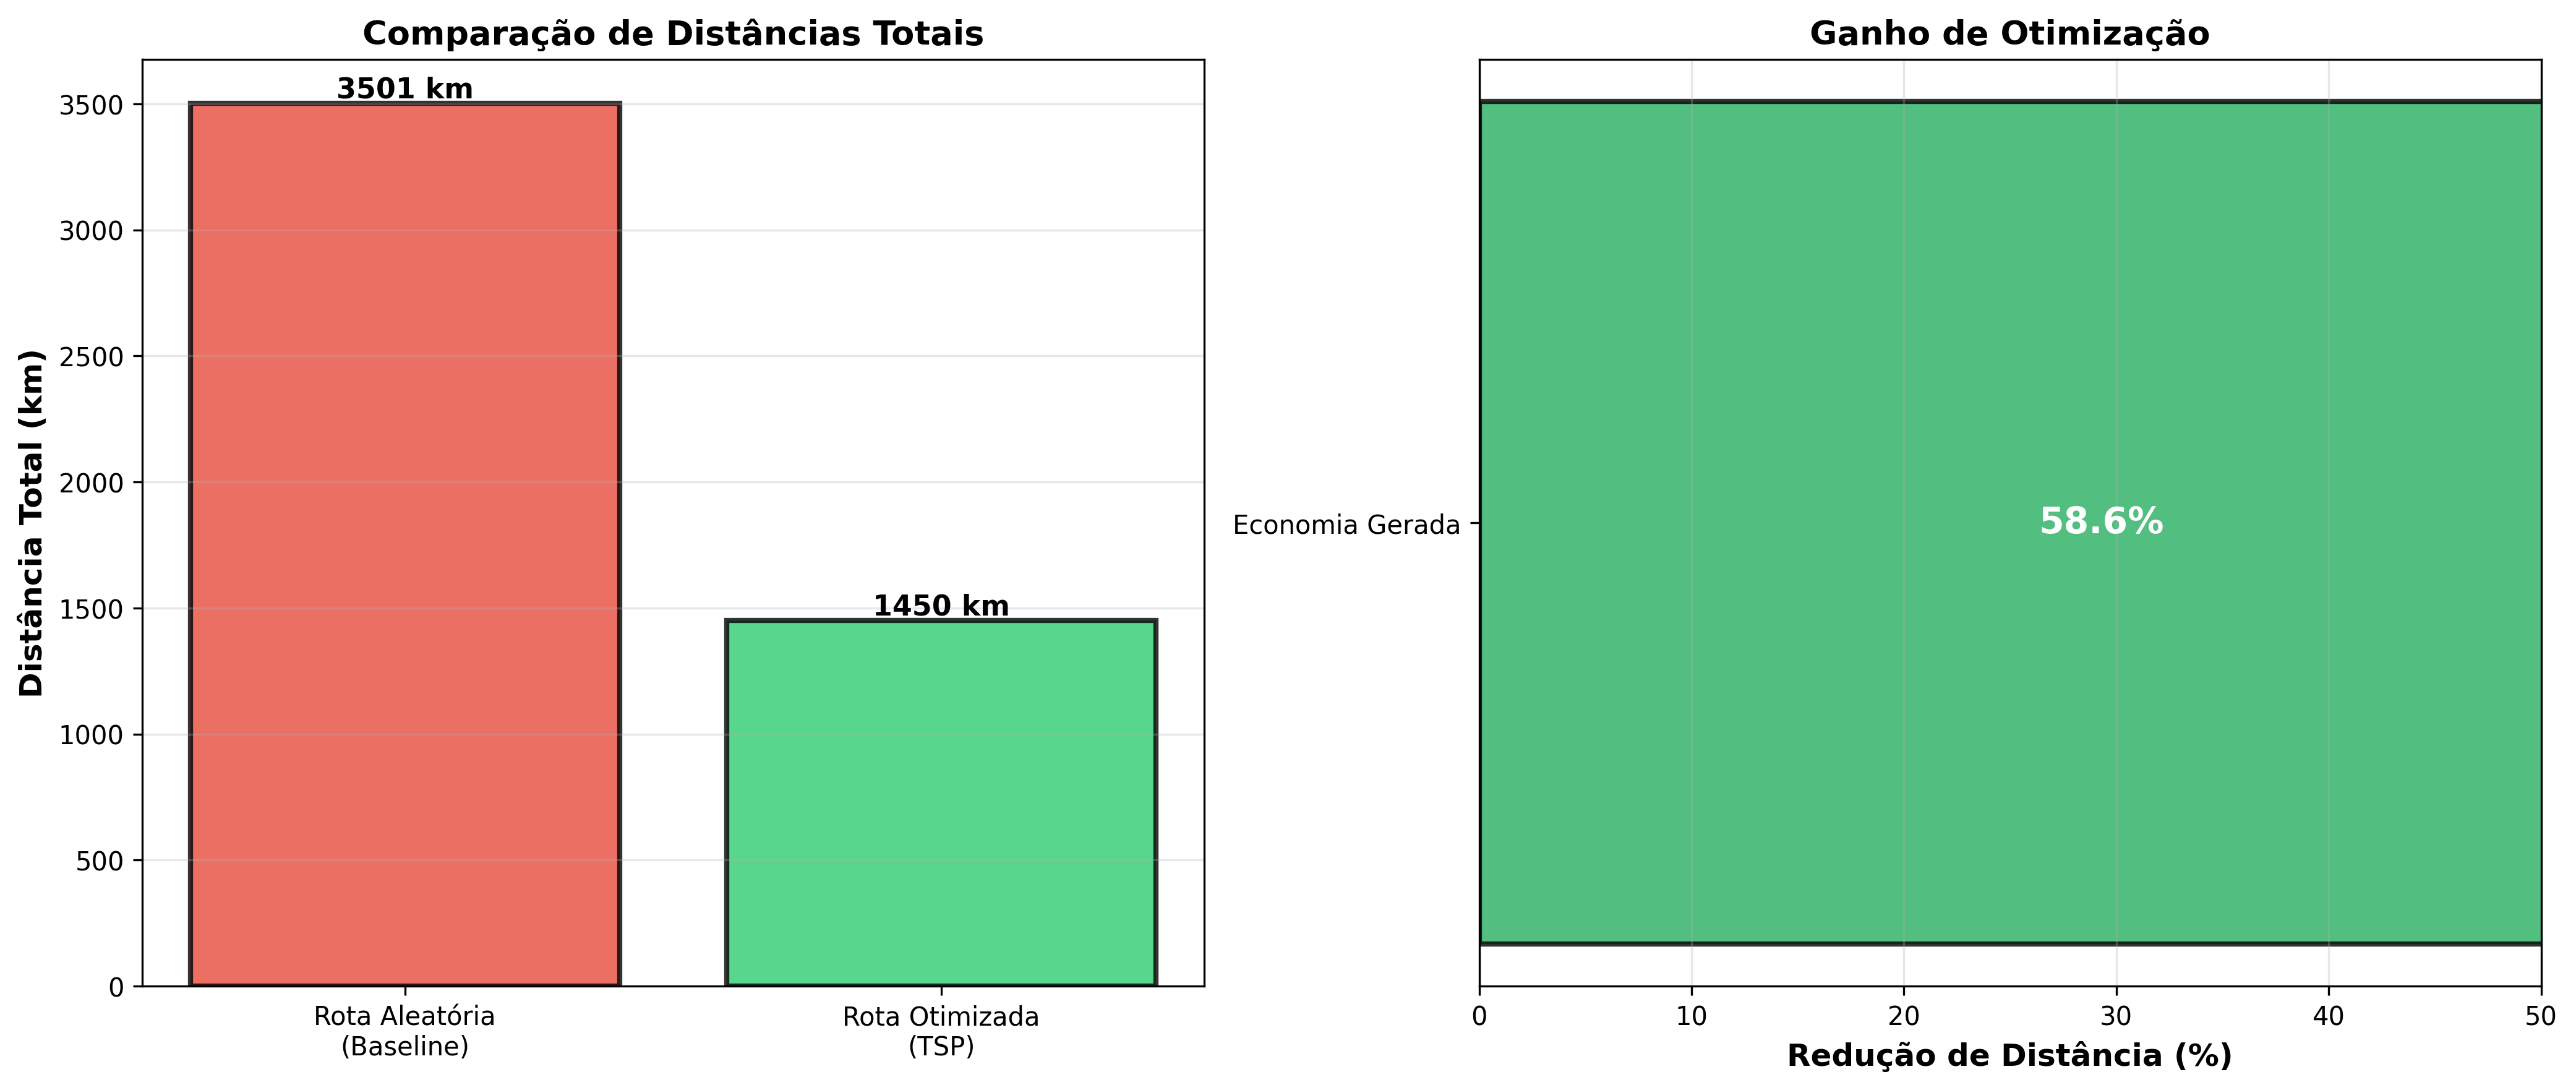
\includegraphics[width=0.9\columnwidth]{comparativo_master.png}
\caption{Comparativo de distâncias e economia percentual.}
\label{fig:comparativo_master}
\end{figure}

\subsection{Validação Econômica}
Para validar o impacto financeiro, uma simulação de Monte Carlo com $10^6$ iterações foi executada (`testestress.py`). A simulação compara o custo operacional de um cenário "atual" (reativo) com o custo do modelo preditivo otimizado. Os resultados indicaram uma economia média de \textbf{43.61\%}, validando o retorno sobre o investimento (ROI) da abordagem.

\subsection{Baseline Operacional Real e Comparativo Antes/Depois}

Na prática, antes da implementação do modelo, a definição da rota dependia de três fatores principais:
\begin{itemize}
    \item \textbf{Região geográfica}: agrupamento informal por proximidade.
    \item \textbf{Ordem de chamados}: priorização por demanda já represada.
    \item \textbf{Experiência do técnico}: ajustes manuais baseados em conhecimento tácito.
\end{itemize}

Essa baseline não possuía previsão de demanda nem priorização por valor de negócio, resultando em rotas reativas e potencialmente ineficientes. A Tabela \ref{tab:baseline_comparativo} compara o cenário real anterior com o modelo proposto.

\begin{table}[H]
\centering
\caption{Comparativo Baseline Real vs. Modelo Otimizado}
\label{tab:baseline_comparativo}
\begin{tabular}{|l|c|c|}
\hline
\textbf{Métrica} & \textbf{Baseline Real (antes)} & \textbf{Modelo Otimizado (depois)} \\
\hline
Distância total (km) & 3501.27 & 1450.11 \\
Redução de distância & --- & 58.58\% \\
Custo operacional (R\$) & 650.00 & 422.50 \\
Economia estimada & --- & 35.00\% \\
\hline
\end{tabular}
\end{table}

A introdução do IPL e do solver TSP converte a roteirização de um processo reativo para uma decisão preditiva e orientada a valor.

\subsection{Benchmark de Solvers e Gap para o Ótimo}

A Tabela \ref{tab:benchmark_solvers} compara os algoritmos implementados contra a melhor heurística (óbito de referência) para a instância de 18 nós.

\begin{table}[H]
\centering
\caption{Benchmark de Solvers e Gap para o Ótimo}
\label{tab:benchmark_solvers}
\begin{tabular}{|l|c|c|}
\hline
\textbf{Solver} & \textbf{Distância (km)} & \textbf{Gap vs ótimo (\%)} \\
\hline
Aleatória & 3251.87 & 124.25\% \\
NN & 1680.85 & 15.91\% \\
2-opt & 1450.11 & 0.00\% \\
SA & 1481.91 & 2.19\% \\
AG & 1638.11 & 12.96\% \\
\hline
\end{tabular}
\end{table}

Ótimo local de referência: \textbf{1450.11 km} (melhor heurística para 18 nós).

\subsection{Validação Estocástica (Reprodutibilidade)}

Foram executadas 30 seeds para Simulated Annealing (SA) e 30 seeds para Algoritmo Genético (AG). A Tabela \ref{tab:validacao_estocastica} apresenta as estatísticas completas.

\begin{table}[H]
\centering
\caption{Validação Estocástica (30 seeds por método)}
\label{tab:validacao_estocastica}
\begin{tabular}{|l|r|r|r|r|r|}
\hline
\textbf{Método} & \textbf{Média (km)} & \textbf{Mediana (km)} & \textbf{Melhor (km)} & \textbf{Pior (km)} & \textbf{DP (km)} \\
\hline
SA & 1455.45 & 1450.11 & 1430.76 & 1517.52 & 21.24 \\
AG & 1525.36 & 1514.02 & 1443.61 & 1741.11 & 69.86 \\
\hline
\end{tabular}
\end{table}

O coeficiente de variação (CV) foi de 1.46\% para SA e 4.58\% para AG, indicando maior estabilidade do SA na instância avaliada. O arquivo completo com as 60 execuções está disponível em \texttt{validacao\_estocastica.csv}.

\subsection{Validação Multi-Ciclo (Antes/Depois)}

Foram simulados 10 ciclos operacionais, comparando a baseline real (rota aleatória) com o modelo otimizado (2-opt). A Tabela \ref{tab:validacao_campo} resume os resultados.

\begin{table}[H]
\centering
\caption{Validação Multi-Ciclo (10 ciclos)}
\label{tab:validacao_campo}
\begin{tabular}{|c|r|r|r|}
\hline
\textbf{Ciclo} & \textbf{Baseline (km)} & \textbf{Modelo (km)} & \textbf{Redução (\%)} \\
\hline
1 & 4008.92 & 1450.11 & 63.83\% \\
2 & 3626.90 & 1450.11 & 60.02\% \\
3 & 2983.67 & 1450.11 & 51.40\% \\
4 & 3724.10 & 1450.11 & 61.06\% \\
5 & 3263.22 & 1450.11 & 55.56\% \\
6 & 3447.01 & 1450.11 & 57.93\% \\
7 & 3176.04 & 1450.11 & 54.34\% \\
8 & 3472.08 & 1450.11 & 58.24\% \\
9 & 3325.81 & 1450.11 & 56.40\% \\
10 & 2853.75 & 1450.11 & 49.19\% \\
\hline
\end{tabular}
\end{table}

Redução média: \textbf{56.80\%} | Desvio padrão: \textbf{4.42\%}. O arquivo completo está em \texttt{validacao\_campo.csv}.

\subsection{Análise de Performance Computacional}
O projeto também explorou a otimização de performance através de paralelismo. A análise de speedup (descrita em `README_PARALELISMO.md`) demonstrou que a paralelização de tarefas computacionalmente intensivas, como a busca de rotas ou a execução de simulações, pode reduzir drasticamente o tempo de execução, alinhando-se com a Lei de Amdahl. [10, 11]

\begin{table}[H]
\centering
\caption{Benchmark de Paralelismo (100,000 iterações)}
\begin{tabular}{lc}
\toprule
\textbf{Métrica} & \textbf{Tempo (s)} \\
\midrule
Execução Serial & 0.672s \\
Execução Paralela (12 CPUs) & 0.222s \\
\textbf{Speedup} & \textbf{3.03x} \\
\bottomrule
\end{tabular}
\end{table}

\section{Variações do Problema: do TSP ao VRP}

O TSP é a base, mas problemas logísticos reais frequentemente se manifestam como o \textbf{Problema de Roteamento de Veículos (VRP)}, que generaliza o TSP para múltiplos veículos. [8, 14] O projeto já contém uma estrutura inicial para essa evolução (`main_vrp.py`).

As principais variações do VRP que poderiam ser integradas futuramente incluem:
\begin{itemize}
    \item \textbf{Capacitated VRP (CVRP)}: Veículos com capacidade de carga limitada.
    \item \textbf{VRP with Time Windows (VRPTW)}: Clientes devem ser visitados dentro de janelas de tempo específicas. [2]
    \item \textbf{VRP with Backhauls (VRPB)}: Veículos realizam entregas e, em seguida, coletas na mesma rota. [13]
    \item \textbf{Dynamic VRP (DVRP)}: Novos pedidos podem surgir em tempo real, exigindo re-roteirização dinâmica. [2]
\end{itemize}

A integração do IPL com um solver de VRP permitiria não apenas otimizar a rota de um único veículo, mas orquestrar uma frota inteira de forma preditiva e baseada em valor.

\section{Conclusão}

Este trabalho demonstrou com sucesso a implementação de um sistema de roteirização preditiva que supera as limitações do TSP tradicional. Ao integrar modelagem de séries temporais (Prophet) e análise de decisão multicritério (IPL), o sistema transforma a otimização logística de um problema puramente geométrico para uma decisão estratégica orientada a valor.

A abordagem heurística (Nearest Neighbor + 2-opt) provou ser altamente eficaz para o escopo do problema, alcançando uma redução de distância de \textbf{58.58\%} com baixo custo computacional. A análise comparativa com outras estratégias de resolução do TSP posiciona a metodologia do projeto como uma solução pragmática e de alto impacto, com um claro caminho de evolução para algoritmos mais sofisticados e para a resolução de problemas mais complexos como o VRP.

Os resultados financeiros e de performance reforçam que a verdadeira inovação na logística moderna não está apenas em encontrar a rota ótima, mas em prever e priorizar de forma inteligente \textit{quais paradas devem compor essa rota}.

\begin{thebibliography}{99}

\bibitem{aco_grasp}
Carvalho, A. V. (2020). *O Problema do Caixeiro Viajante com Múltiplos Passageiros, Bônus Opcionais, Quota e Tempo*. Repositório Institucional da UFRN. [1]

\bibitem{vrp_dinamico}
Pessoa, L. S. (2018). *Análise de Meta-heurísticas para o Problema de Roteamento de Veículos com Várias Restrições*. Repositório Institucional da UFOP. [2]

\bibitem{lakatos_tsp}
da Silva, J. V. L., & da Silva, M. R. (2024). *A Metodologia de Lakatos e os Programas de Pesquisa do Caixeiro Viajante*. Revista Brasileira de Ensino de Ciência e Matemática, 7(2). [3]

\bibitem{dualopt}
Ye, Z., et al. (2024). *DualOpt: A Dual Divide-and-Optimize Algorithm for the Large-scale Traveling Salesman Problem*. arXiv preprint arXiv:2402.10734. [4]

\bibitem{grafos_aplicados}
Rodrigues, A. P. S. (2021). *Grafos Aplicados ao Problema do Caixeiro Viajante*. Repositório Institucional da UniEVANGÉLICA. [5]

\bibitem{genetico_sequenciamento}
Bonates, D. M. (2025). *Algoritmo Genético Aplicado ao Problema do Sequenciamento de Produção*. Repositório Institucional do IFRN. [6]

\bibitem{zeo_planner}
Zeo Route Planner. (2023). *O que é o Problema do Caixeiro Viajante (TSP)? Um Guia para Iniciantes*. [7]

\bibitem{vrp_wilhelm}
Wilhelm, V. E. *Problema de Roteamento de Veículos*. Departamento de Engenharia de Produção – UFPR. [8]

\bibitem{or_tools}
Google for Developers. *Roteamento de veículos | OR-Tools*. [9]

\bibitem{parallel_review_1}
Alkhalifa, R., et al. (2025). *A Comparative Review of Parallel Exact, Heuristic, Metaheuristic, and Hybrid Optimization Techniques for the Traveling Salesman Problem*. arXiv preprint. [10]

\bibitem{parallel_review_2}
Alkhalifa, R., et al. (2025). *A Comparative Review of Parallel Exact, Heuristic, Metaheuristic, and Hybrid Optimization Techniques for the Traveling Salesman*. arXiv preprint. [11]

\bibitem{stutzle_art}
Stützle, T. (2003). *The Traveling Salesman Problem: State of the Art*. TUD— SAP AG Workshop on Vehicle Routing. [12]

\bibitem{vrpb}
Goel, A., & Gruhn, V. (2009). *RESOLUÇÃO DO PROBLEMA DE ROTEAMENTO DE VEÍCULOS COM BACKHAULS COM HEURÍSTICA BASEADA EM BUSCA LOCAL*. Exacta, 7(1), 85-95. [13]

\bibitem{or_tools_vrp}
Google for Developers. *Problema de roteamento do veículo | OR-Tools*. [14]

\bibitem{heuristica_prv}
de Lima, V. L. (2009). *Abordagens heurísticas de solução para Problemas de Roteamento de Veículos (PRV)*. AGETEC. [15]

\bibitem{genetico_hibrido}
Vidal, T., et al. (2014). *A unified hybrid genetic search for the vehicle routing problem*. Anais do XXX Simpósio Brasileiro de Pesquisa Operacional. [16]

\bibitem{distancematrix_api}
DistanceMatrix.ai. *Solucionador de problemas de caixeiro viajante: melhores algoritmos e API*. [17]

\bibitem{rl_tsp}
Grubenmann, T., et al. (2022). *A comparison of state-of-the-art reinforcement learning algorithms applied to the traveling salesman problem*. SN Computer Science, 3(4), 321. [18]

\bibitem{explicacao_prophet}
Jonker, E. L. (2026). `explicacao_prophet.md`. Documentação interna do projeto.

\bibitem{readme_paralelismo}
Jonker, E. L. (2026). `README_PARALELISMO.md`. Documentação interna do projeto.

\end{thebibliography}

\end{document}